%%%%%%%%%%%%%%%%%%%%%%%%%%%%%%%%%%%%%%%%%%%%%%
%                                            %
%   W Z O R Z E C   S P R A W O Z D A N I A  %
%                                            %
%%%%%%%%%%%%%%%%%%%%%%%%%%%%%%%%%%%%%%%%%%%%%%


\documentclass[12pt,a4paper,twoside]{article}

\usepackage{amsmath,amssymb}
\usepackage[utf8]{inputenc}                                      
\usepackage[OT4]{fontenc}      
%\usepackage[T1]{fontenc}                            
\usepackage[polish]{babel}                           
\selectlanguage{polish}
\usepackage{indentfirst} 
\usepackage[dvips]{graphicx}
\usepackage{tabularx}
\usepackage{color}
\usepackage{hyperref} 
\usepackage{fancyhdr}
\usepackage{listings}
\usepackage{booktabs}
\usepackage{ifpdf}
\usepackage{mathtext} % polskie znaki w trybie matematycznym
%\makeindex  % utworzenie skorowidza (w dokumencie pdf)
\usepackage{lmodern}
%\usepackage[osf]{libertine}
\usepackage{filecontents}
\usepackage{ifthen}


\usepackage{tikz}
\usetikzlibrary{arrows}


\newcounter{nextYear}
\setcounter{nextYear}{\the\year}
\stepcounter{nextYear}

% rozszerzenie nieco strony
%\setlength{\topmargin}{-1cm} \setlength{\textheight}{24.5cm}
%\setlength{\textwidth}{17cm} \addtolength{\hoffset}{-1.5cm}
%\setlength{\parindent}{0.5cm} \setlength{\footskip}{2cm}
%\linespread{1.2} % odstep pomiedzy wierszami


%%%% ZYWA PAGINA %%%%%%%%%%%
\newcommand{\tl}[1]{\textbf{#1}} 
\pagestyle{fancy}
\renewcommand{\sectionmark}[1]{\markright{\thesection\ #1}}
\fancyhf{} % usuwanie bieżących ustawień
\fancyhead[LE,RO]{\small\bfseries\thepage}
\fancyhead[LO]{\small\bfseries\rightmark}
\fancyhead[RE]{\small\bfseries\leftmark}
\renewcommand{\headrulewidth}{0.5pt}
\renewcommand{\footrulewidth}{0pt}
\addtolength{\headheight}{0.5pt} % pionowy odstęp na kreskę
\fancypagestyle{plain}{%
\fancyhead{} % usuń p. górne na stronach pozbawionych numeracji
\renewcommand{\headrulewidth}{0pt} % pozioma kreska
}

%%%%%   LISTINGI %%%%%%%%
% ustawienia listingu programow

\lstset{%
language=C++,%
commentstyle=\textit,%
identifierstyle=\textsf,%
keywordstyle=\sffamily\bfseries, %
%captionpos=b,%
tabsize=3,%
frame=lines,%
%numbers=left,%
numberstyle=\tiny,%
numbersep=5pt,%
breaklines=true,%
morekeywords={pWezel,Wezel,string,ref,params_result},%
escapeinside={(*@}{@*)},%
%basicstyle=\footnotesize,%
%keywords={double,int,for,if,return,vector,matrix,void,public,class,string,%
%float,sizeof,char,FILE,while,do,const}
}
%%%%%%%%%%%%%%%%%%%%%%%%%%%%%%%%%%%%%%%%%%%%%%%%%%%%%%%%%%%%%%%%%%%%%%%

%%%%%%%%%  NOTKI NA MARGINESIE %%%%%%%%%%%%%
% mala zmiana sposobu wyswietlania notek bocznych
\let\oldmarginpar\marginpar
\renewcommand\marginpar[1]{%
  {\linespread{0.85}\normalfont\scriptsize%
\oldmarginpar[\hspace{1cm}\begin{minipage}{3cm}\raggedleft\scriptsize\color{black}\textsf{#1}\end{minipage}]%    left pages
{\hspace{0cm}\begin{minipage}{3cm}\raggedright\scriptsize\color{black}\textsf{#1}\end{minipage}}% right pages
}%
}
% % % % % % % % % % % % % % % % % % % % % % % % % % % % % % % %

%%%% WYSWIETLANIE AKTUALNEGO ROKU AKADEMICKIEGO %%%%%%%%%%%
\newcounter{rok}
\newcommand{\rokakademicki}{%
   \setcounter{rok}{\number\year}%
   \ifthenelse{\number\month<10}%
   {\addtocounter{rok}{-1}}% rok akademicki zaczal sie w pazdzierniku poprzedniego roku
   {}%                       rok akademicki zaczyna sie w pazdzierniku tego roku
   \arabic{rok}/\addtocounter{rok}{1}\arabic{rok}
}
%%%%%%%%%%%%%%%%%%%%%%%%%%%%%%%%%%%%%%%


%%%% LISTA UWAG %%%%%%%%%
\usepackage{color}
\definecolor{brickred}      {cmyk}{0   , 0.89, 0.94, 0.28}

\makeatletter \newcommand \kslistofremarks{\section*{Uwagi} \@starttoc{rks}}
\newcommand\l@uwagas[2]
{\par\noindent \textbf{#2:} %\parbox{10cm}
   {#1}\par} \makeatother


\newcommand{\ksremark}[1]{%
   {{\color{brickred}{[#1]}}}%
   \addcontentsline{rks}{uwagas}{\protect{#1}}%
}

\newcommand{\comma}{\ksremark{przecinek}}
\newcommand{\nocomma}{\ksremark{bez przecinka}}
\newcommand{\styl}{\ksremark{styl}}
\newcommand{\ortografia}{\ksremark{ortografia}}
\newcommand{\fleksja}{\ksremark{fleksja}}
\newcommand{\pauza}{\ksremark{pauza `--', nie dywiz `-'}}
\newcommand{\kolokwializm}{\ksremark{kolokwializm}}
\newcommand{\cytowanie}{\ksremark{cytowanie}}

%%%%%%%%%%%%%%%%%%%%%%%%%
%%%%%%%%%%%%%%%%%%%%%%%%%
%%%%%%%%%%%%%%%%%%%%%%%%%
%%%%%%%%%%%%%%%%%%%%%%%%%
%%%%%%%%%%%%%%%%%%%%%%%%%
%%%%%%%%%%%%%%%%%%%%%%%%%
%%%%%%%%%%%%%%%%%%%%%%%%%
%%%%%%%%%%%%%%%%%%%%%%%%%
%%%%%%%%%%%%%%%%%%%%%%%%%
%%%%%%%%%%%%%%%%%%%%%%%%%
%%%%%%%%%%%%%%%%%%%%%%%%%
%%%%%%%%%%%%%%%%%%%%%%%%%



% autor:
\fancyhead[RE]{\small\bfseries Broncel, Nieora} % autor sprawozdania



%%%%%%%%%%% NO I ZACZYNA SIE SPRAWOZDANIE %%%%%%%%%%%

\begin{document}
\frenchspacing
\thispagestyle{empty}
\begin{center}
{\Large\sf Politechnika Śląska   % Alma Mater

Wydział Automatyki, Elektroniki i Informatyki

}

\vfill

 

\vfill\vfill

{\Huge\sffamily\bfseries Implementacja switcha SDN na banana PI R2\par}  

\vfill\vfill

{\LARGE\sf }   


\vfill \vfill\vfill\vfill

%%%%%%%%%%%%%%%%%%%%%%%%%%%%





\begin{tabular}{ll}
	\toprule
	skład sekcji:	&	Rafał Broncel\\
					&	Jan Nieora\\
	kierunek:		& Informatyka\\
	grupa: 			& ISMiP1 \\
	
	\bottomrule
	                            &
\end{tabular}

\end{center}
%%% koniec strony  tytulowej

%%%%%%%%%%%%%%%%%%%%%%%%%%%%%%%%%%%%%%%%%%%%%%%%%%%%%%%%%%%%%%%%%%%%%%%%%
\cleardoublepage
%%%%%%%%%%%%%%%%%%%%%%%%%%%%%%%%%%%%%%%%%%%%%%%%%%%%%%%%%%%%%%%%%%%%%%%%%

%%%%%%%%%%%%%%%%%%%%%%%%%%%%%%%%%%%%%%%%%%%%%%%%%%%%%%%%%%%%%%%%%%%%%%%%%

%%%%%%%%%%%%%%%%%%%%%%%%%%%%%%%%%%%%%%%%%%%%%%%%%%%%%%%%%%%%%%%%%%%%%%%%%
\section{Opis projektu}
W celu zrealizowania  switch'a SDN na banana PI R2 wykorzystaliśmy system operacyjny \texttt{Armbian 21.03}. Dodatkowo w roli kontrolera wykorzystaliśmy program \texttt{Opendaylight} w wersji \texttt{karaf 08.04} wraz z zewnętrzną nakładka graficzną \texttt{OpenflowApp}. Kontroler był uruchomony na komputerze z systemem \texttt{Ubuntu 20.04}. Dodatkowo w celu łatwiejszej konfiguracji oraz przepływu pakietów \texttt{OpenFlow} wykorzystaliśmy zew. kartę sieciową podłączoną do gniazda USB.
\section{uruchomienie i konfiguracja kontrolera}
W celu uruchomienia \texttt{Opendaylight'a} należy pobrać środowisko \texttt{JAVA 8 JRE}.
Następnie wystarczy rozpakować skompresowany folder i uruchomić program poleceniem: \texttt{./karaf-0.8.4/bin/karaf}.
Konieczne jest zainstalowanie trzech podstawowych features'ów: 
\begin{itemize}
	\item\texttt{odl-openflowplugin-app-topology-manager}  
	\item\texttt{odl-l2switch-all}
	\item\texttt{odl-restconf-all}
\end{itemize}
W celu uruchomienia nakładki graficznej należy wejść do pobrango folderu z Open \texttt{OpenflowApp} i wykonać polecenie \texttt{grunt}. Następnie w przeglądarce uruchomić stronę:
 \url{http://localhost:9000}. Przeglądarka  powinna pokazać strone przedstawiona na rysunku \ref{OFM}.
 \begin{figure}[!h]
 	\centering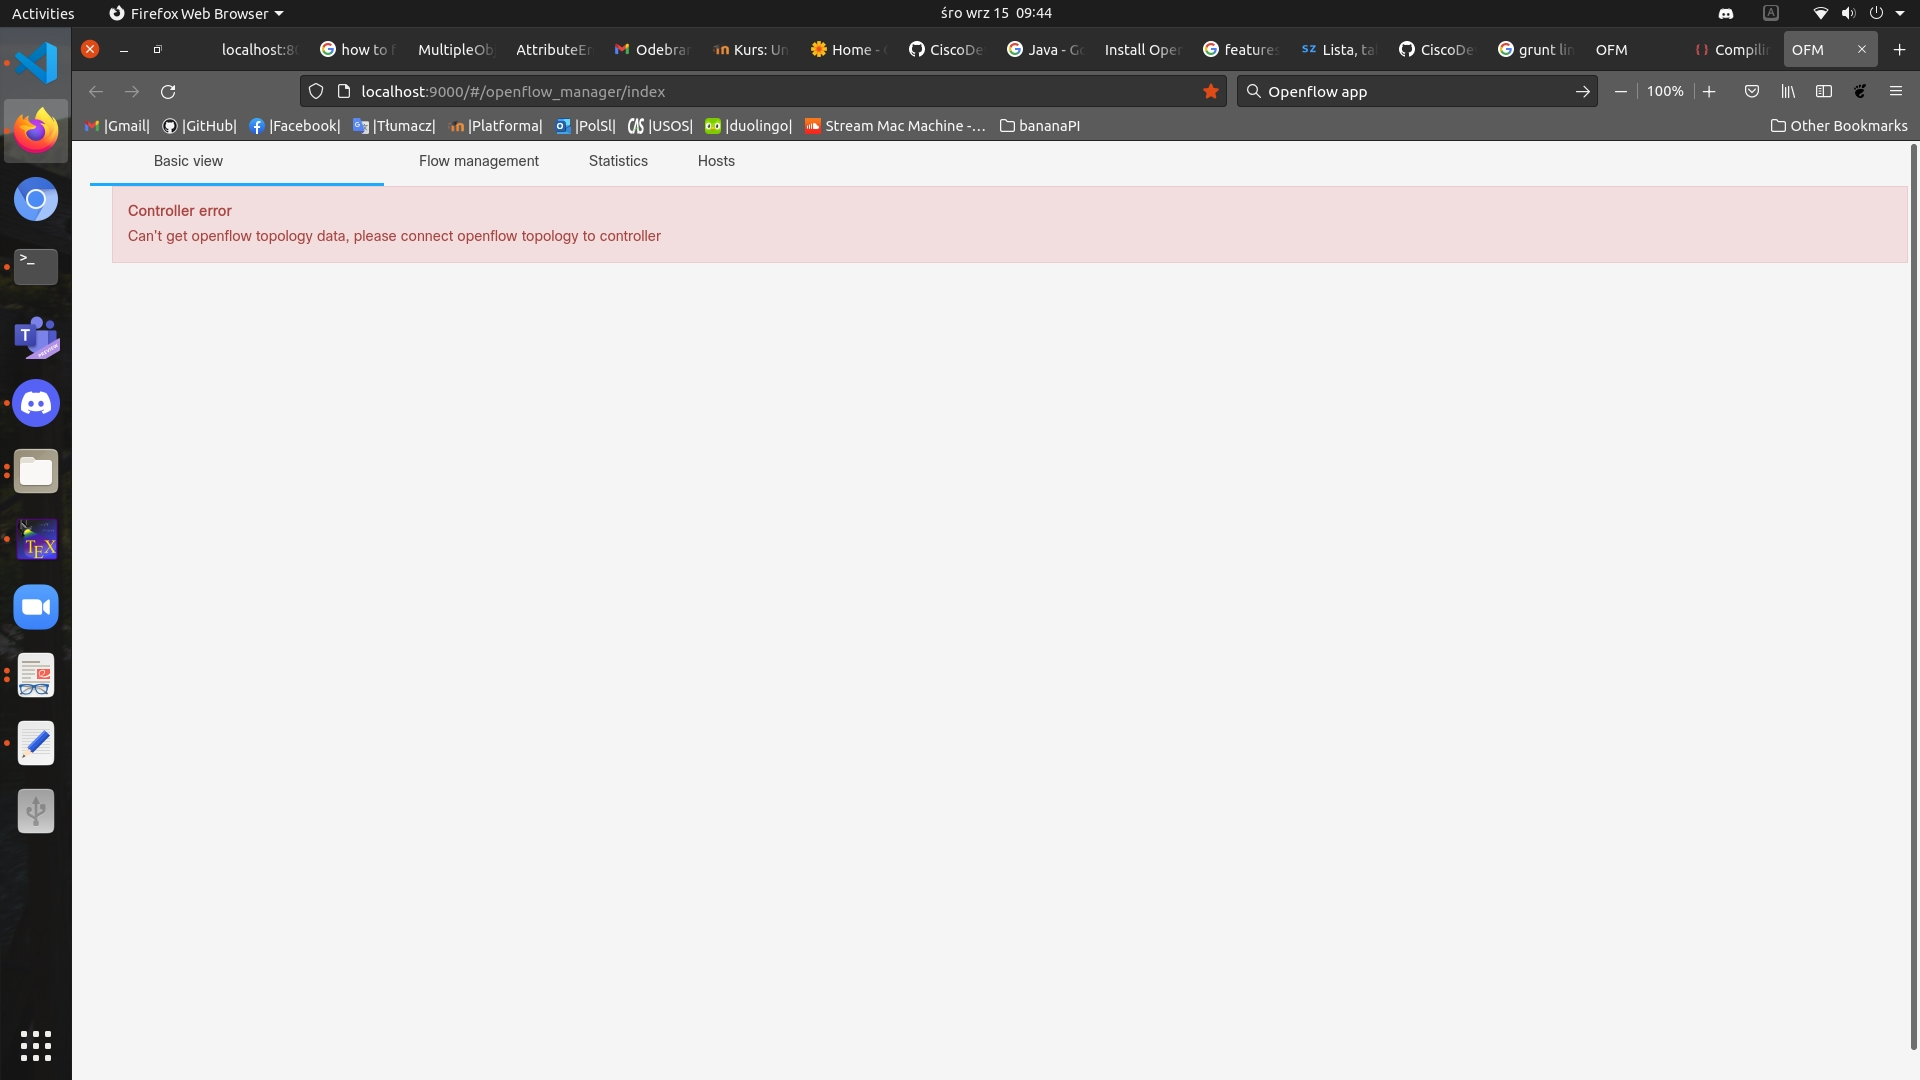
\includegraphics[width=0.7\textwidth]{OFM_uruchomienie.jpg}
 	\caption{Uruchomienie nakładki graficznej bez uruchomionego banana PI R2} \label{OFM}
 \end{figure}
\newline Po powyższych korkach ODL z OFM powinny być poprawnie skonfigurowane.


\section{Uruchomienie i konfiguracja banana PI R2}
Po zgraniu systemu na kartę sd należy podłączyć urządzenie do sieci w celu znalezienia banana pi'a wykorzystaliśmy 
polecenie \texttt{nmap} należy znać sieć i jej maskę. Rysunek \ref{nmap} przedstawia wykonanie polecenia w domowej sieci 

\begin{figure}[!h]
	\centering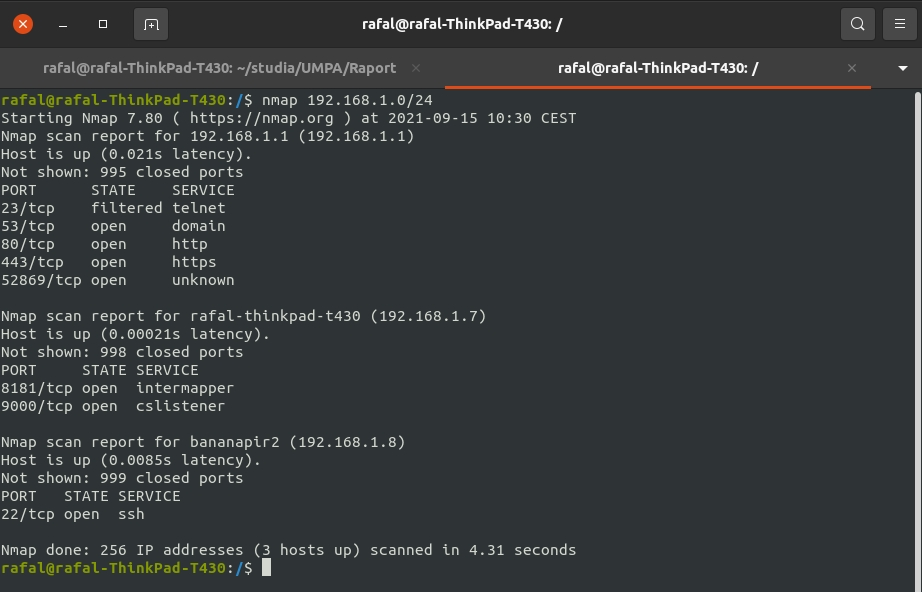
\includegraphics[width=0.7\textwidth]{nmap.jpg}
	\caption{Uruchomienie polecenia nmap} \label{nmap}
\end{figure}

W mojej sieci polecenie określa który adres ip należy do urządzenia, niestety w niektórych sieciach tak się nie dzieje więc trzeba zwracać uwagę na otwarte porty w przypadku banana pi'a  otwarty jest tylko port 22. Aby się połączyć z urządzeniem należy wykonać polecenie: \texttt{ssh root@<adres ip banana pi>}. Po połączeniu możemy przystąpić do konfiguracji. 
\par Pierwszym krokiem jest zainstalowanie \texttt{Open vSwitch}'a. Po instalacji musimy stworzyć most oraz ustawić adres ip kontrolera. , co jest pokazane poniżej:
\begin{itemize}
	\item\texttt{ovs-vsctl add-br br1}  
	\item\texttt{ovs-vsctl set-controller br1 tcp:<adres ip kontrolera>}
\end{itemize}

Po tych krokach ODL powinien wykryć banana pi'a jako switch'a.Przeglądarka z włączonym OFM na adresie \url{http://localhost:9000} powinna przedstawiać podobny widok tak jak rysunek \ref{OFM_banana}
 
 \begin{figure}[!h]
 	\centering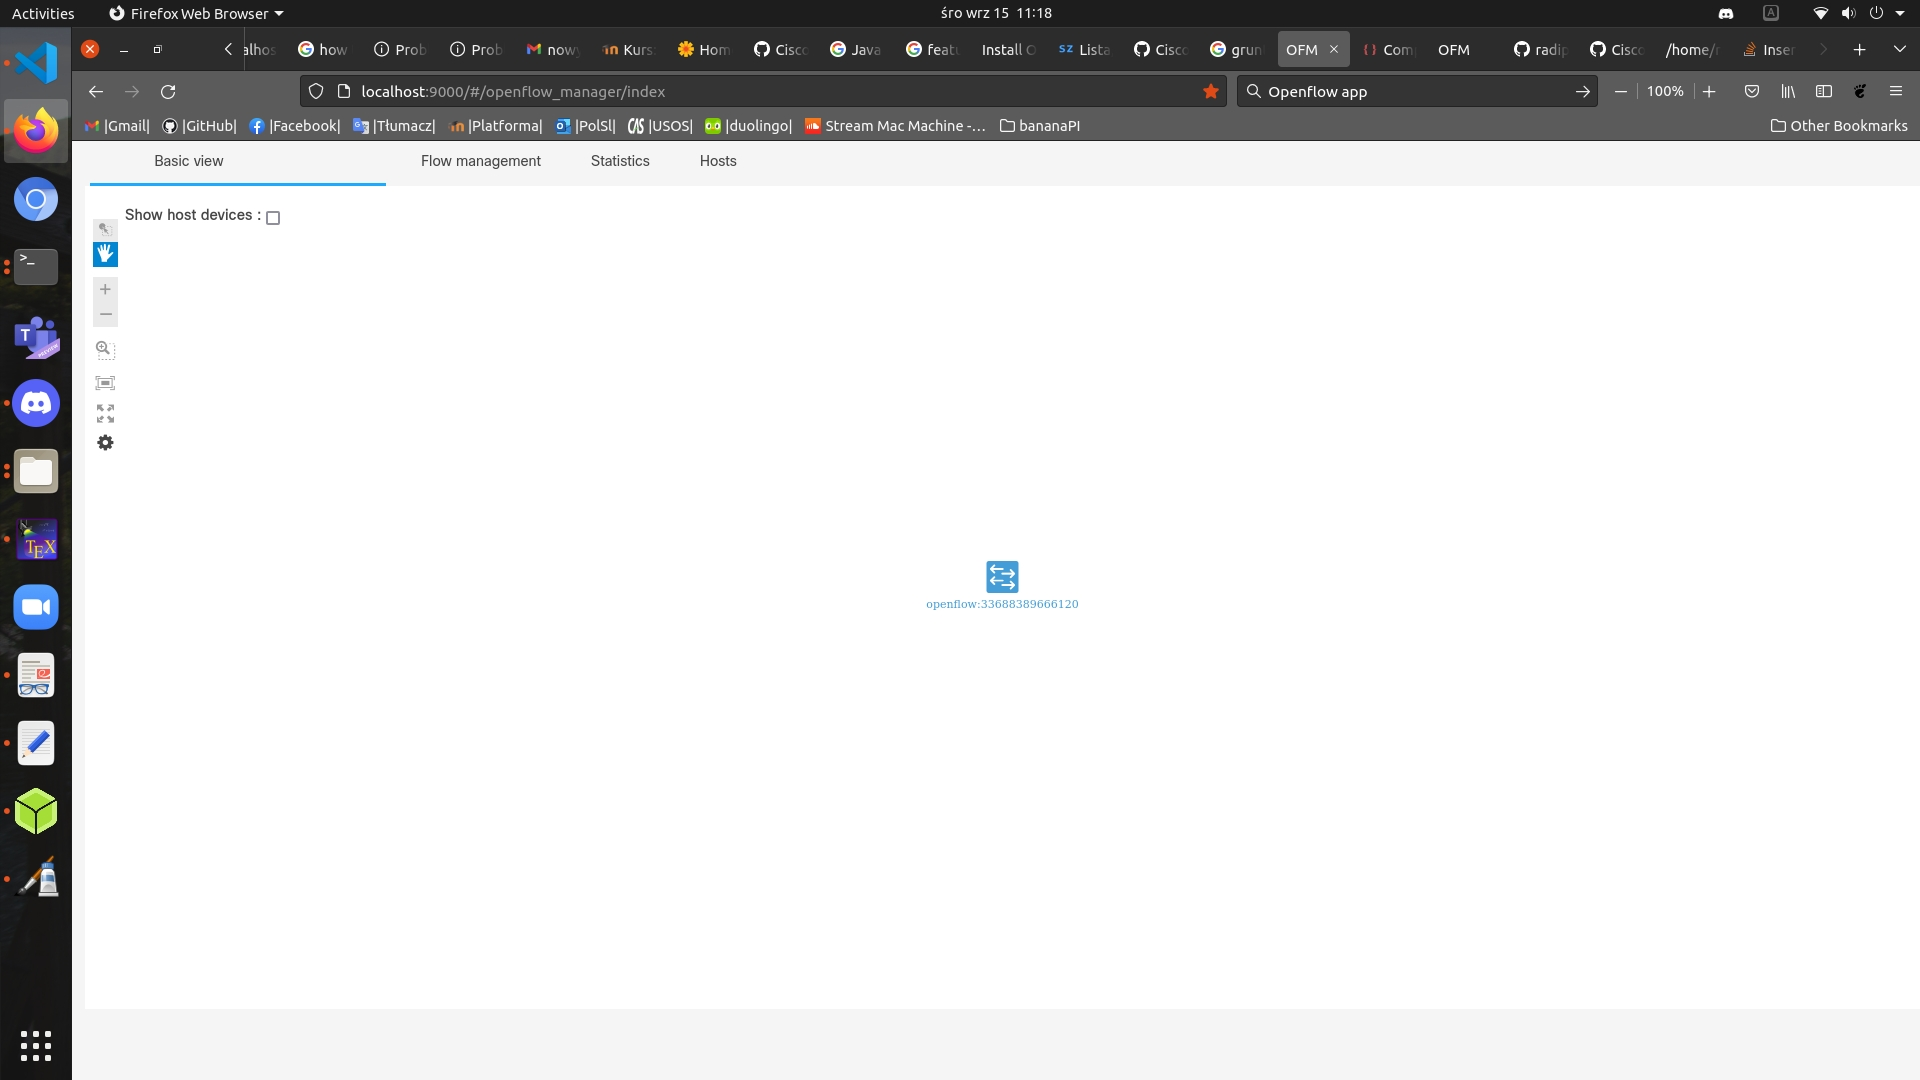
\includegraphics[width=1\textwidth]{OFM_banana.jpg}
 	\caption{Uruchomienie banana PI z wstępnie skonfigurowanym swatchem } \label{OFM_banana}
 \end{figure}
 \newpage
\par Kolejnym korkiem jest uruchomienie poniższego skryptu, który musi byc uruchamiany za każdym razem jeśli banana pi nie zapamiętał ustawień, niestety nie zawsze zapamiętuje ustawienia. 

\begin{lstlisting}

ip link set dev wan down 
ip link set dev  eth0 down
ip link set dev wan address ca:fe:ca:fe:ca:fe
sudo ip link set dev eth0 address 12:12:12:12:12:12
ip link set dev wan up



#split eth0

ip link set eth0 up
ip link add link eth0 name eth0.10 type vlan id 10
ip link add link eth0 name eth0.20 type vlan id 20
ip link add link eth0 name eth0.30 type vlan id 30
ip link add link eth0 name eth0.40 type vlan id 40
ip link add link eth0 name eth0.50 type vlan id 50


ip link set dev eth0.10 down 
ip link set dev eth0.20 down 
ip link set dev eth0.30 down 
ip link set dev eth0.40 down 
ip link set dev eth0.50 down 

#change mac 

ip link set dev eth0.10  address 12:12:12:12:12:10
ip link set dev eth0.20  address 12:12:12:12:12:20 
ip link set dev eth0.30  address 12:12:12:12:12:30 
ip link set dev eth0.40  address 12:12:12:12:12:40 
ip link set dev eth0.50  address 12:12:12:12:12:50  

ip link set lan0 address ca:fe:ca:fe:ca:c0
ip link set lan1 address ca:fe:ca:fe:ca:c1
ip link set lan2 address ca:fe:ca:fe:ca:c2
ip link set lan3 address ca:fe:ca:fe:ca:c3



ip link set dev wan up



#remove

bridge vlan del vid 1 dev lan0
bridge vlan del vid 1 dev lan1
bridge vlan del vid 1 dev lan2
bridge vlan del vid 1 dev lan3
bridge vlan del vid 1 dev wan


#correct tag

bridge vlan add vid 10 dev lan0 pvid untagged
bridge vlan add vid 20 dev lan1 pvid untagged
bridge vlan add vid 30 dev lan2 pvid untagged
bridge vlan add vid 40 dev lan3 pvid untagged
bridge vlan add vid 50 dev wan pvid untagged 


#turn on


ip link set dev br0 up
ip link set eth0.10 up
ip link set eth0.20 up
ip link set eth0.30 up
ip link set eth0.40 up
ip link set eth0.50 up

ip link set lan0 nomaster
ip link set lan1 nomaster
ip link set 
\newpagelan2 nomaster
ip link set lan3 nomaster
ip link set wan nomaster


ip link set wan up
ip link set lan0 up
ip link set lan1 up
ip link set lan2 up
ip link set lan3 up
\end{lstlisting}






Teraz przechodzimy do konfiguracji samego \texttt{Open vSwitch}'a
Po wyonaniu skryptu możemy przejśc do konfiguracji switcha. W tym celu musimy na początku wyłączyc lan'y i eth. W tym celu wykonujemy następujące komendy (które wystarczy uruchomic jednorazowo): 

\begin{verbatim}
ip link set dev eth0	down 
ip link set dev eth0.10 down 
ip link set dev eth0.20 down 
ip link set dev eth0.30 down 
ip link set dev eth0.40 down 
ip link set dev eth0.50 down 

ip link set wan  down
ip link set lan0 down
ip link set lan1 down
ip link set lan2 down
ip link set lan3 down
\end{verbatim}

Kolejnym krokiem jest dodanie powyższych interfejsów do \texttt{Open vSwitch}'a wieć trzeba wykonać nastepujące polecenia: 

\begin{verbatim}
ovs-vsctl add-port br1 eth0.10
ovs-vsctl add-port br1 eth0.20 
ovs-vsctl add-port br1 eth0.30
ovs-vsctl add-port br1 eth0.40
ovs-vsctl add-port br1 eth0.50

ovs-vsctl add-port br1 wan
ovs-vsctl add-port br1 lan0
ovs-vsctl add-port br1 lan1
ovs-vsctl add-port br1 lan2
ovs-vsctl add-port br1 lan3
\end{verbatim}

Następnie musimy włączyc interfejsy:
\begin{verbatim}
ip link set dev eth0	up
ip link set dev eth0.10 up
ip link set dev eth0.20 up
ip link set dev eth0.30 up
ip link set dev eth0.40 up
ip link set dev eth0.50 up

ip link set wan  up
ip link set lan0 up
ip link set lan1 up
ip link set lan2 up
ip link set lan3 up
\end{verbatim}

Po powyzszych krokach możemy wykonac polecnie \texttt{ovs-vsctl show}, które powinno nam przedstawic podbny rezultat
co rysunek \ref{ovs}. Tym samym powinismy mieć w pełni skonfigurowanego switcha. Istotnym faktem jest to, że switch wykryje tylko urządzenia jeśli przejdze przez niego jaki kolwiek ruch sieciowy z urządzenia. Wystarczy użyc polenia \texttt{ping} na dowoly adres ip. Kolejną ważnym szczegółem jest fakt, że jesli będzemy blokować cały ruch to banana pi nie wykryje nowych urządzeń. 

 \begin{figure}[!h]
	\centering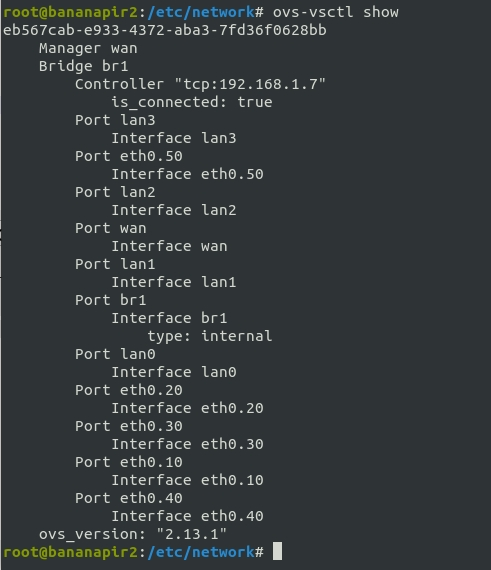
\includegraphics[width=1\textwidth]{ovs_show.jpg}
	\caption{Skonfigurowany ovs}
	\label{ovs}
\end{figure}

\newpage
Rysunek \ref{Dev} przestawia główny widok OFM'a który świadczy o porawnej konfiguracji i otym że switch wykrył podłączone urządzenia.  


\begin{figure} [!h]
	\centering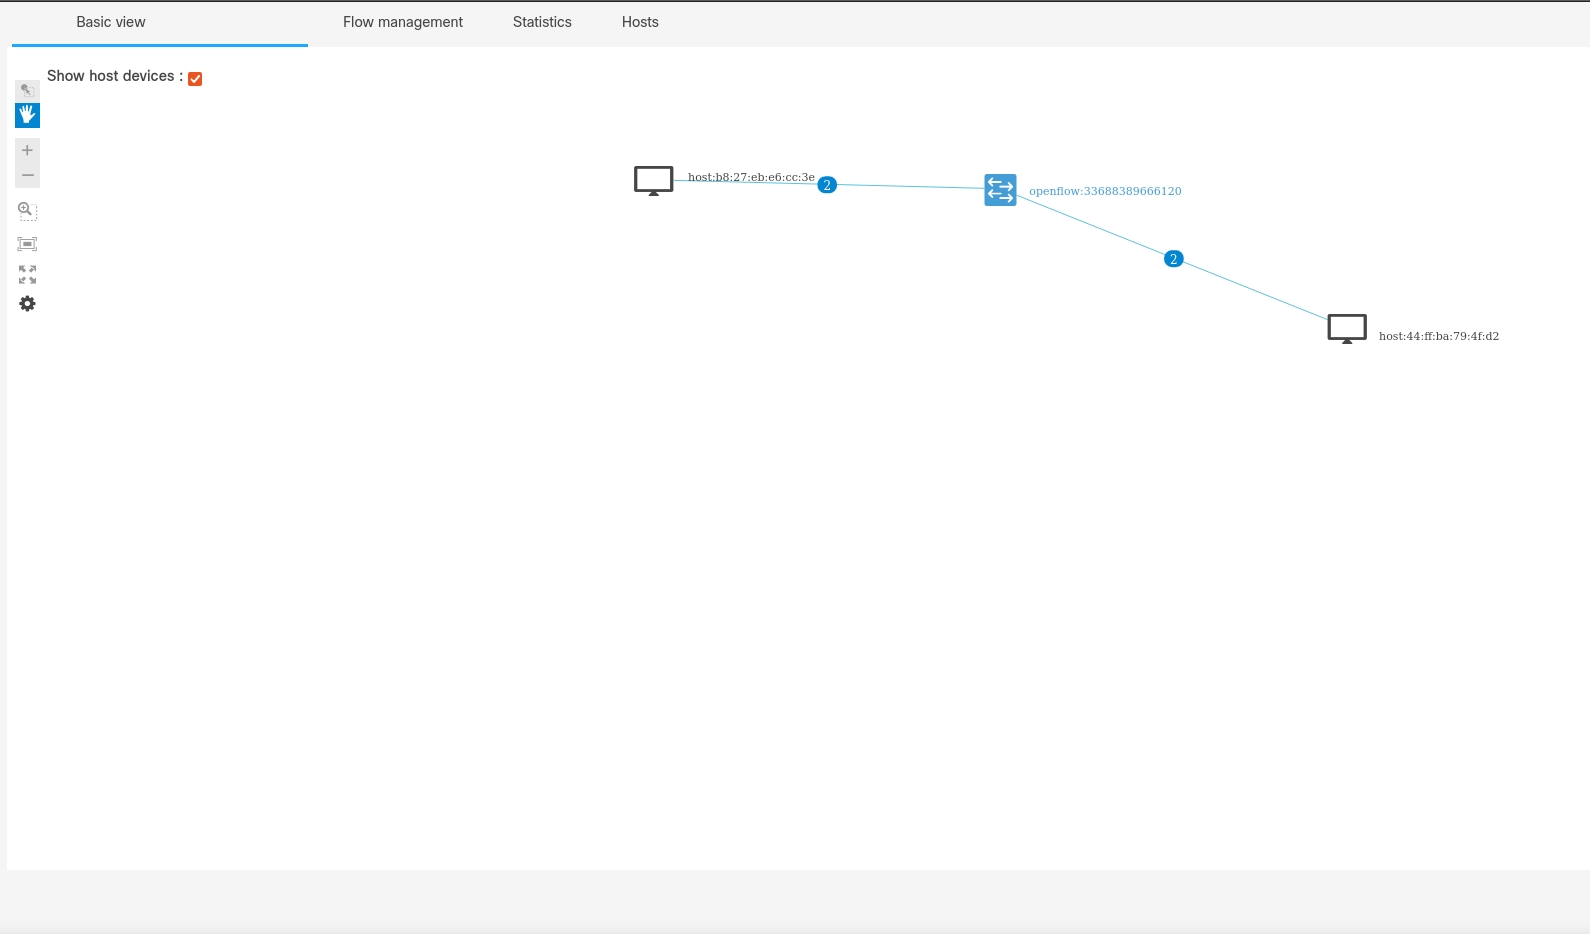
\includegraphics[width=1\textwidth]{Dev.jpg}
	\caption{Dev}
	\label{Dev}
\end{figure}


\section{Uwagi końcowe i wnioski}
\begin{itemize}
	\item Deklaracja przepływów z wykorzystaniem adresów ip nie działa, poporostu takie przepływy nie chcą się zapisać, jest to ogólnie zany problem w internecie, niestety nie znaleźliśmy rozwiązania. 
	\item Aby switch widział urządzenia konieczne jest wymuszenie przepływu pakietów.
	\item Podczas uruchomienia pierwszego przepływu mija nawet kilka sekund zanim switch zacznie działać.
	\item Aby switch mógł mieć dostęp do internetu i jednocześnie mieć kontakt z kontrolerem należy używać zewnętrzej karty sieciowe, która umożliwi przepływ pakietów \texttt{OpenFlow}. W tym przypadku do portu wan można podpiąć sieć i tym samym urządzenia dostają adresy ip z puli sieci.
	\item W przypadku gdy do portu wan nie podłączymy sieci.
	\item System Armbian nie wspiera obsługi wewnętrznego modułu wi-fi. Doszukaliśmy się informacji, że urzywając zewnętrzych modułów wi-fi podłączonych do gniazda usb są szanse aby uruchomić wi-fi na banana pi. 
	\item Odrzuciliśmy system OpenWRT, ponieważ nie posiadał bibliotek potrzebnych do zainstalowania OVS'a.
	\item Podczas tworzenia projektu mieliśmy wrażenie, że większość rzeczy jest przestarzałych i ogólnie nie wspieranych.
	\item Banana Pi działa bardzo nie stabilenie, czasem po restarcie trzeba uruchamiać skrypt konfigurujący porty lan, a czasem nie.
	\item Zewnętrzną karta sieciowa jest konieczna, aby w łatwy sposób konfigurować ustawienia sieciowe.
	
\end{itemize}

Zewnetrzna karta sieciowa jest konieczna aby w łatwy sposób konfigurować ustawienia sieciowe. 

\section*{Żródła}

\begin{itemize}
	\item \href{https://john.soban.ski/install-opendaylight-ubuntu-lts-fast.html}{Istalacja Javy wraz z uruchomieniem ODL}
	\item \href{https://github.com/CiscoDevNet/OpenDaylight-Openflow-App}{OFM}
\end{itemize}

\end{document}
% Koniec wieńczy dzieło.
